\documentclass{article}

\usepackage[romanian]{babel}
\usepackage[a4paper]{geometry}
\usepackage[hidelinks]{hyperref}
\usepackage[section]{placeins}
\usepackage{fancyhdr}
\usepackage{graphicx}
\usepackage{microtype}

\graphicspath{ {../images/} }

\title{{\huge Sokoban}\\Tema 1 - Inteligență Artificială}
\author{Alexandru Sima (332CA)}

\begin{document}

\maketitle
\begin{abstract}
    Analiza a 2 strategii de rezolvare a jocului de Sokoban prin explorarea 
    spațiului stărilor: \textbf{Beam Search} și \textbf{Learning Real-Time A*}. 
    Prezentarea unei soluții de rezolvare și evaluarea performanțelor, comparând
    cele 2 strategii, cât și prezentarea raționamentului care a condus la 
    această soluții și comparații cu idei anterioare.
\end{abstract}

\pagestyle{fancy}
\lhead{\textit{Sokoban - Tema 1 IA}}
\rhead{\textit{Alexandru Sima - 332CA}}

\newpage
\tableofcontents

\newpage
\section{Introducere}
Sokoban este un joc puzzle, care constă într-o zonă de joc pătrată, împărțită în
celule. Celulele pot fi goale sau blocate de pereți. În celulele goale se află 
un jucător și un număr egal de cutii și ținte. Jucătorul se poate deplasa în 
cele 4 celule adiacente, dacă nu sunt blocate de pereți. Acesta poate și împinge
cutiile, dacă sunt pe direcția de deplasare și (ca o relaxare a regulilor), le 
poate și trage înapoi.

Scopul jocului este de a muta fiecare cutie pe câte o țintă diferită, evitând, 
pe cât posibil, tragerile.

\begin{figure}[ht]
    \begin{center}
        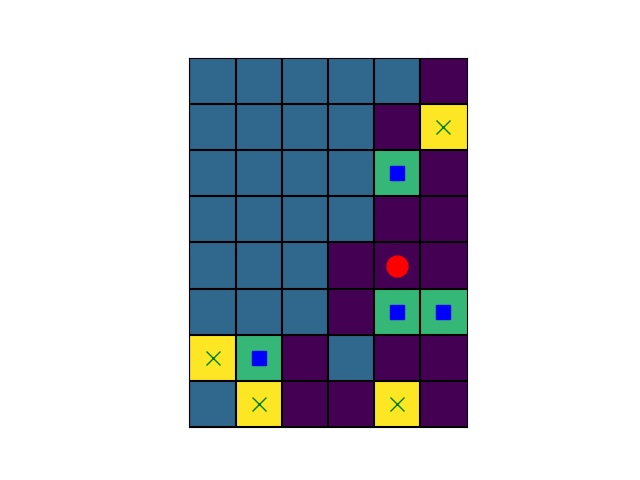
\includegraphics[scale=0.7]{hard_map1.png}
    \end{center}
    \caption{Exemplu de hartă Sokoban. Jucătorul trebuie să mute cutiile vezi 
    în celulele țintă (galbene). Pereții sunt marcați cu albastru.}
    \label{fig:sokoban}
\end{figure}

\section{Soluție propusă}
Soluția folosește o euristică relativ simplă, reușind să rezolve toate testele
în mai puțin de 6 secunde și fără a trage cutii. 

\subsection{Beam Search}
Algoritmul funcționează după cum urmează: se pleacă de la o stare inițială,
care va reprezenta \textit{beamul} inițial; la fiecare pas, se expandează 
vecinii fiecărei stări din \textit{beam}, se elimină duplicatele și se 
calculează costul fiecărei stări, conform euristicii, apoi se aleg următoarele 
$k$ stări pentru a forma noul \textit{beam}. Pentru a evita anumite situații
în care algoritmul se blochează în niște minime locale ale funcției de cost, 
am ales o abordare stocastică: nu se aleg cele mai bune $k$ stări, ci $k$ stări 
cu o probabilitate care ia în calcul costul stării (aplicând softmax pe 
costurile obținute).

Algoritmul poate fi ajustat prin:
\begin{itemize}
    \item \textit{heuristic}: funcție care estimează costul unei stări;
    \item \textit{state\_generator}: funcție care generează vecinii unei stări;
    \item \textit{max\_iters}: numărul maxim de iterații ale \textit{beamului}
    până la care se încearcă rezolvarea;
    \item \textit{k}: dimensiunea \textit{beamului}.    
\end{itemize}

\subsection{Learning Real-Time A*}
Algoritmul, ca și cel precedent, pornește dintr-o stare inițială și, la fiecare
pas, evaluează vecinii stării în care se află și avansează înspre cel de cost 
minim. Pentru a învăța costurile (și a converge spre costurile reale), se rețin 
într-o tabelă asocieri $(stare \rightarrow cost)$. Aceasta se populează cu 
valori când se evaluează o stare nemaiîntâlnită (se introduce costul estimat de 
euristică) și la fiecare tranziție între stări (fiind cel mai bun cost cunoscut,
se consideră că este mai aproape de adevăr). Deoarece, când nu este permis ca
jucătorul să tragă cutii, pot exista stări de deadlock (în care jocul este 
pierdut), dacă, după un număr stabilit de pași, algoritmul nu găsește o stare cu
un cost mai bun, la fiecare pas va avea o probabilitate să se întoarcă într-o 
stare anterioară (reținând tabela de estimări, pentru a o îmbunătăți mai 
departe).

Algoritmul poate fi ajustat prin:
\begin{itemize}
    \item \textit{heuristic}: funcție care estimează costul unei stări;
    \item \textit{state\_generator}: funcție care generează vecinii unei stări;
    \item \textit{max\_iters}: numărul maxim de mișcări din starea inițială până
    la care se încearcă rezolvarea;
    \item \textit{backoff\_steps}: numărul de pași înapoi efectuați la primul 
    backoff;
    \item \textit{backoff\_steps\_increment}: numărul de pași cu care se mărește
    lungimea backoffului după fiecare astfel de eveniment;
    \item \textit{backoff\_probability\_factor}: factor care influențează 
    probabilitatea de backoff;
    \item \textit{cost\_plateau\_treshold}: numărul de pași fără o îmbunătățire
    a costului după care se încearcă backoffuri.
\end{itemize}

\subsection{Euristica propusă}

Funcția de cost aleasă pentru algoritmii de căutare este suma distanțelor de la
cutii la pătrățelele țintă. Pentru fiecare cutie, se calculează distanța 
(în împingeri) către fiecare pătrățel de pe hartă (și, implicit, către fiecare 
țintă), apoi se asociază fiecărei cutii o țintă, astfel încât suma distanțelor 
să fie minimă. Împerechearea se face cu ajutorul \textit{Hungarian method}.

\subsection{Analiza performanțelor}\label{sec:performances}

Parametri utilizați:
\begin{itemize}
    \item Parametri comuni:
    \begin{itemize}
        \item \textit{heuristic}: Manhattan
        \item \textit{state\_generator}: mutări fără trageri
    \end{itemize}
    \item Beam Search:
    \begin{itemize}
        \item \textit{max\_iters}: 200
        \item \textit{k}: 80
    \end{itemize}
    \item Learning Real-Time A*:
    \begin{itemize}
        \item \textit{max\_iters}: 20000
        \item \textit{backoff\_steps}: 10
        \item \textit{backoff\_steps\_increment}: 10
        \item \textit{backoff\_probability\_factor}: 0.98
        \item \textit{cost\_plateau\_treshold}: 20
    \end{itemize}
\end{itemize}

Rulând algoritmii pe setul de teste furnizat, se observă următoarele tipare:

\subsubsection*{Timpul de execuție}
Timpul de execuție pentru algoritmul Beam Search este semnificativ mai mare
decât cel pentru Learning Real-Time A*, datorită nevoii de a evalua vecinii 
tuturor stărilor din beam la fiecare pas (\textit{lungime\_beam} $\cdot$ 
\textit{număr\_vecini} $\approx k \cdot 4$); LRTA*, pe de altă parte, consideră
doar starea curentă și vecinii acesteia. Se poate observa în (\ref{fig:time}) că
LRTA* este chiar și cu un ordin de mărime mai rapid decât Beam Search pentru 
aproape toate testele. O excepție evidentă este testul "\textit{large\_map2}"
(\ref{fig:large_map_2}), in care, cel mai probabil, LRTA* efectuează un număr 
mult prea mare de backoffuri, deoarece sunt multe stări similare din punct de 
vedere al costului.

\begin{figure}[ht]
    \begin{center}
        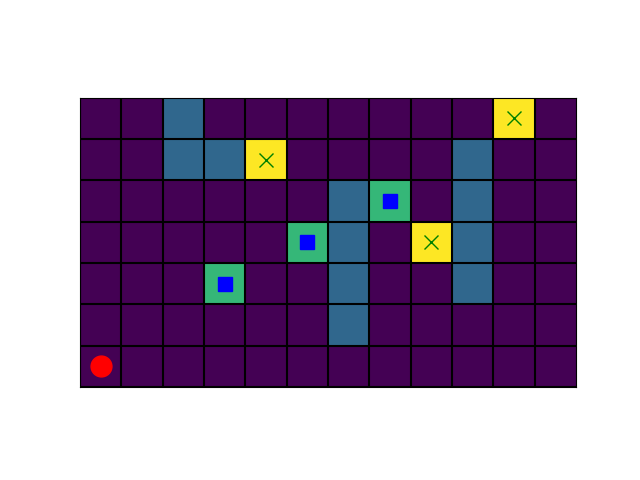
\includegraphics[scale=0.4]{large_map2.png}
    \end{center}
    \caption{Testul "\textit{large\_map2}"}
    \label{fig:large_map_2}
\end{figure}

\begin{figure}[ht]
    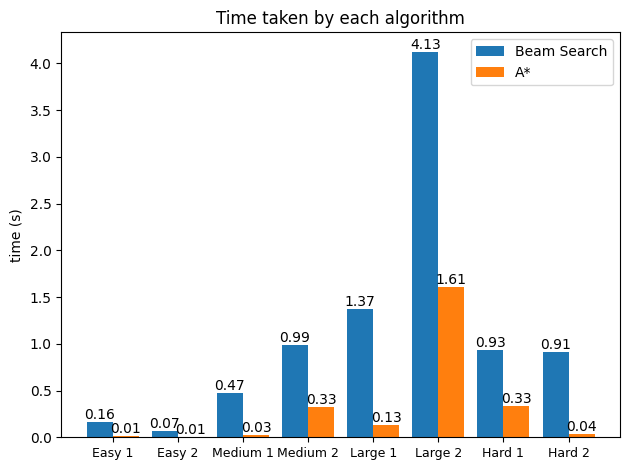
\includegraphics[scale=0.55]{solution/time.png}
    \caption{Timpul de execuție al algoritmilor pe diferite teste}
    \label{fig:time}
\end{figure}

\subsubsection*{Numărul de stări vizitate}
Numărul de stări evaluate urmează, din aceleași considerente, un tipar similar.
Se remarcă în (\ref{fig:explored_states}) însă un număr similar de stări 
evaluate în testul "\textit{hard\_map1}" (\ref{fig:hard_map1}), care are o 
soluție foarte puțin evidentă, ceea ce conduce la multe backoffuri în cazul 
LRTA*.

\begin{figure}[ht]
    \begin{center}
        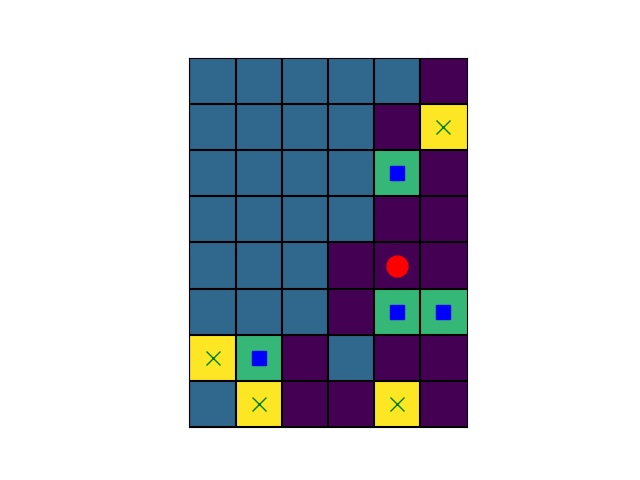
\includegraphics[scale=0.4]{hard_map1.png}
    \end{center}
    \caption{Testul "\textit{hard\_map1}"}
    \label{fig:hard_map1}
\end{figure}

\begin{figure}[ht]
    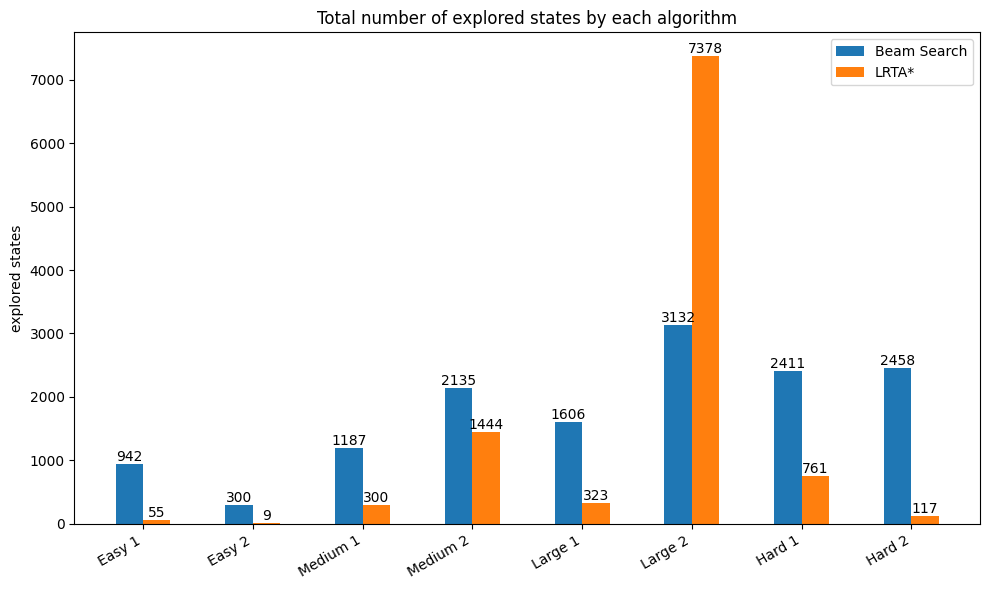
\includegraphics[scale=0.55]{solution/explored_states.png}
    \caption{Numărul de stări vizitate de algoritmi în cazul fiecărui test}
    \label{fig:explored_states}
\end{figure}

\subsubsection*{Optimalitatea soluției}
Conform rezultatelor din (\ref{fig:solution_length}), Beam Search găsește 
soluții mai scurte decât LRTA*, deoarece cel din urmă poate să se întoarcă în 
stări anterioare pentru că învață în timp real costurile stărilor. 

\begin{figure}[ht]
    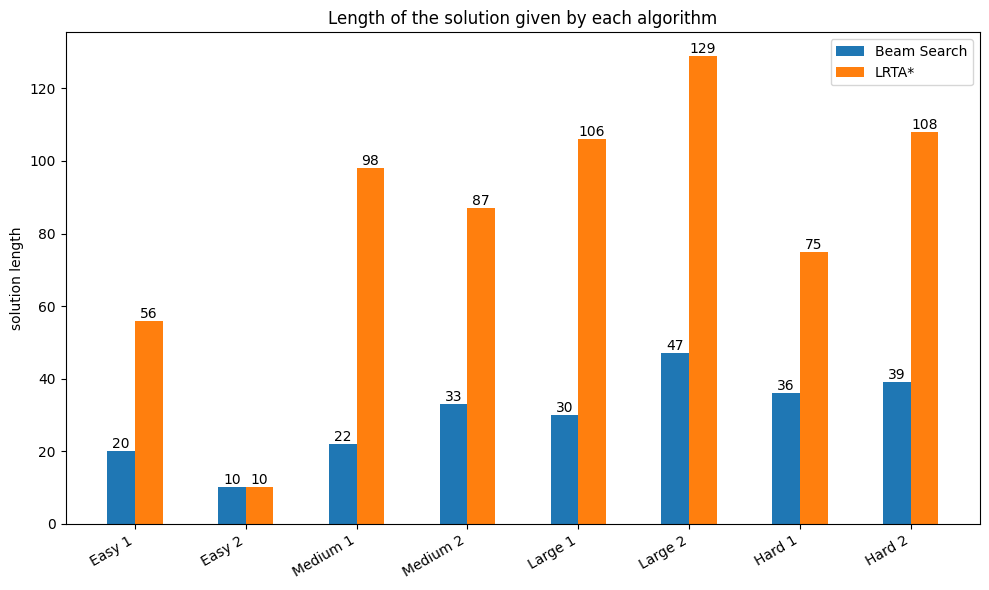
\includegraphics[scale=0.55]{solution/solution_length.png}
    \caption{Lungimea soluției (numărul de mișcări) găsite de algoritmi pentru 
    teste}
    \label{fig:solution_length}
\end{figure}

\section{Raționament}

\subsection{Funcția de cost}

\subsubsection{Distanța Manhattan}
Prima idee de implementare a fost însumarea distanței Manhattan de la fiecare
cutie la cea mai apropiată țintă. Această euristică se calculează foarte ușor și
este \textit{consistentă}, dar nu este foarte eficientă, tendința jucătorului 
fiind să împingă cutiile în direcția țintelor, ignorând existența pereților. 
Pentru a compensa acest fapt, am mărit \textit{beamul} și am ales o abordare
stocastică în alegerea stărilor care să constituie \textit{beamul}. Inițial am
decis să se aleagă $k$ stări cu o probabilitate proporțională cu costul 
fiecăreia (de exemplu, având 3 stări cu costurile 1, 2 și 3, acestea să fie 
alese cu probabilitățile $\frac{3}{6}$, $\frac{2}{6}$, respectiv $\frac{1}{6}$).
Această abordare nu a funcționat, deoarece stărilor cu costuri mari le erau 
atribuite probabilități mult prea mari. Soluția a fost transformarea costurilor
în probabilități cu ajutorul funcției \textit{softmax}, care oferă probabilități
care scad exponențial cu cât costul este la o distanță mai mare de maximum.
Funcția 
\textit{softmax}\footnote{\url{https://en.wikipedia.org/wiki/Softmax_function}}
folosită (\ref{for:softmax}) a suferit mici modificări față de cea originală, 
deoarece am dorit să atribui probabilități mari stărilor cu costuri mici, am 
normalizat valorile $x_i$ în apropierea lui 0 și nu am adăugat un parametru de 
temperatură (care controlează cât de brusc scad probabilitățile odată cu 
distanța, comportându-se similar cu cea din algoritmul \textit{Simulated 
Annealing}).

\begin{figure}[ht]
    \begin{center}
        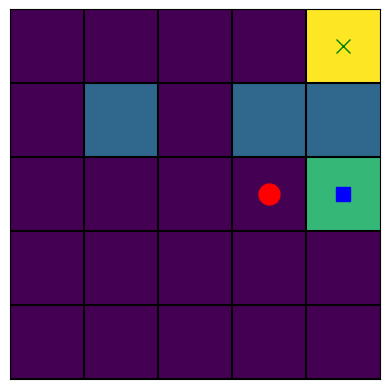
\includegraphics[scale=0.4]{manhattan.png}
    \end{center}
    \caption{Situație în care Beam Search se blochează într-o stare  de minim 
    local, caz în care $k$ trebuie mărit}
\end{figure}

În parametri aleși la \textbf{\ref{sec:performances}}, algoritmii rezolvă în 
medie doar $6/8$ teste.

\begin{figure}[ht]
    \[ P(x_i) = \frac{e^{x_i - \max(x_k)}}{\sum_{j=1}^n e^{x_j - \max(x_k)}} \]
    \caption{Funcția softmax folosită}
    \label{for:softmax}
\end{figure}

\subsubsection{Numărul minim de mutări}\label{sec:min_moves}
Următoarea idee a fost similară cu cea de mai sus, dar cu un calcul mai fidel al
distanțelor (în loc de distanță Manhattan, pentru fiecare cutie se calculează 
numărul de mișcări până la ținte, folosind algoritmul lui 
Lee\footnote{\url{https://www.pbinfo.ro/articole/18589/algoritmul-lui-lee}}), 
apoi se însumează distanțele pentru fiecare cutie. În plus, am adăugat un 
termen care să țină cont de distanța jucătorului față de cutiiile care nu sunt 
pe ținte, dar, pentru un $k$ mic și cu pondere egala cu cea a distanței 
cutiilor, jucătorul putea ajunge "să se teamă" (\ref{fig:scared}) să împingă 
cutiile pe ținte, deoarece în acest mod se "îndepărta" de cutie. Acest 
impediment a putut fi reglat acordând o pondere mai mare distanței cutiilor.

\begin{figure}[ht]
    \begin{center}
        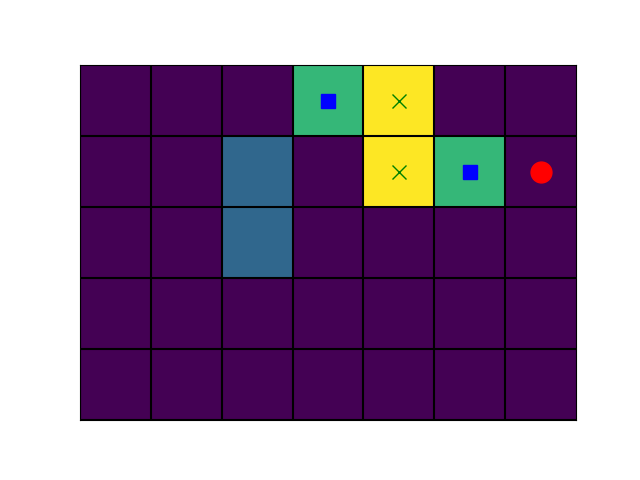
\includegraphics[scale=0.4]{scared.png}
    \end{center}
    \caption{Situație în care s-ar obține un cost mai mare dacă jucătorul ar 
    împinge cutia pe țintă}
    \label{fig:lee}
\end{figure}

\subsubsection{Corespondența cutie - țintă de cost minim}
O evaluare mai apropiată de realitate a numărului de mutări necesare este atinsă
prin asocierea fiecărei cutii cu o țintă. Pentru aceasta, se calculează distanța
de la fiecare cutie la fiecare țintă (similar cu (\ref{sec:min_moves})), apoi se
caută combinația de sumă minimă, folosind 
\textit{Hungarian method}\footnote{\url{https://en.wikipedia.org/wiki/Hungarian_algorithm}}. 
Acesta este deja implementat în \textit{Python} în biblioteca \textit{scipy} 
(\textit{scipy.optimize.linear\_sum\_assignment}).

\subsubsection{Numărul minim de împingeri}
O altă îmbunătățire adusă euristicii a fost ajustarea calculului numărului de 
mutări astfel încât să țină cont dacă acestea sunt posibile (fără trageri).
Varianta finală consideră că o mutare este posibilă dacă atât celula în care se
împinge cutia, cât și cea în care s-ar afla jucătorul sunt libere. Au existat
totuși mai multe variații ale acestei idei, în care am încercat să evit 
deadlock-urile din testele complicate, în special prin restricționarea a ce 
înseamnă "accesibil pentru jucător", însă fără succes. Se remarcă:
\begin{itemize}
    \item O mutare să fie posibilă dacă există o cale fără un zid între jucător
    și poziția de unde trebuie să împingă. Această condiție nu a adus 
    îmbunătățiri semnificative.
    \item O mutare să fie posibilă dacă există o cale fără un zid 
    \underline{sau o altă cutie} între jucător și poziția de unde trebuie să 
    împingă. Această condiție bloca jocul în anumite situații, în special
    în "\textit{hard\_map\_1}".
    \item O mutare să fie cu atât mai costisitoare, cu cât calea de la jucător 
    la poziția de unde trebuie să împingă cutia conține mai multe alte cutii. 
    Similar, aceasta a dus la blocaje în joc.
\end{itemize}

\subsubsection{Distanța până la cutii}
După alegerea euristicii, am încercat îmbunătățirea performanțelor, ținând 
cont, din nou, de distanța jucătorului de cea mai apropiată cutie, dar nu s-a 
dovedit a fi utilă, deoarece a crescut timpul de execuție, fără a aduce soluții
mai bune. Se poate observa în (\ref{fig:comparison}) că lungimea soluțiilor 
rămâne neschimbată pentru Beam Search, iar pentru LRTA* este micșorată doar în 3
situații. Timpul de execuție rămâne aproximativ același pentru LRTA*, dar crește
considerabil în cazul Beam Search.

\begin{figure}[ht]
    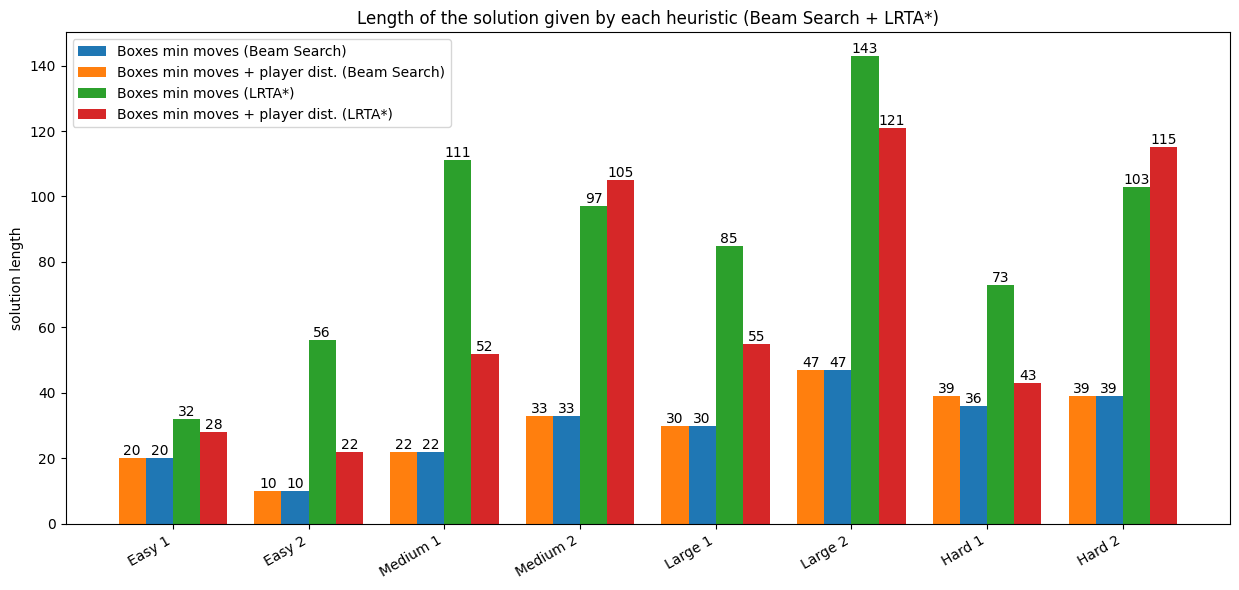
\includegraphics[scale=0.45]{comparison/solution_length.png}
    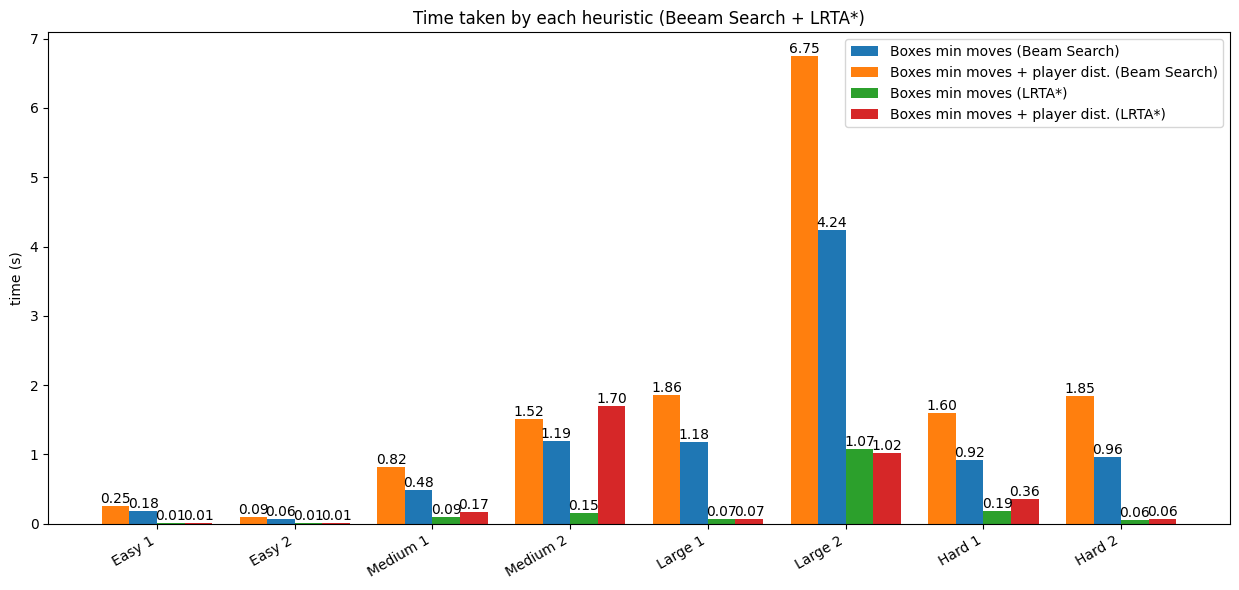
\includegraphics[scale=0.45]{comparison/time.png}

    \caption{Comparație între rezultatele obținute dacă se ține cont sau nu de 
    distanța între jucător și cutii}
    \label{fig:comparison}
\end{figure}

\subsection{Ajustarea LRTA*}
Euristica aleasă s-a dovedit suficient de bună pentru a rezolva testele 
folosind Beam Search, dar nu și pentru LRTA*, deoarece acesta este un algoritm 
online, care poate face mutări care să compromită jocul și efectul acestora să
se simtă mult mai târziu. Pentru a rezolva jocul fără mișcări de \textit{pull},
algoritmul este ajustat să facă \textit{random backoff}: după un număr de mutări
în care nu există nicio îmbunătățire a costului, există o șansă (
crescătoare\footnote{De fapt, se contorizează șansa de a nu se face backoff --- 
inițial 1 --- care scade exponențial atenuat.}) de a se întoarce un număr de 
pași înapoi. Cu fiecare întoarcere, acest număr de pași crește și el (liniar). 
Acești parametri au fost aleși empiric, observând că o întoarcere cu un număr 
constant de pași ar duce la foarte multe întoarceri în testele dificile, iar o 
întoarcere cu un număr de pași care crește exponențial nu ar mai permite 
explorarea stărilor (în special în testele simple).

\section{Concluzii}
Sokoban este un joc cu reguli simple, dar cu o complexitate mare, ceea ce face
ca evaluarea stărilor să fie dificilă. Ambii algoritmi prezentați reușesc să 
rezolve testele propuse, însă fiecare are avantaje și dezavantaje. Beam Search
evaluează mai multe stări promițătoare în paralel, deci are șanse mai mari de 
reușită, chiar și cu o euristică mai puțin informată (precum distanța 
Manhattan), dar evaluează un număr mare de stări și are un timp de execuție 
considerabil; pe de altă parte, LRTA* este mai rapid, dar acesta învață 
costurile pe măsură ce efectuează mutări, ceea ce poate duce la situații 
imposibil de rezolvat dacă subestimează costul anumitor stări. Fără o euristică
foarte bună (pentru a le evita), LRTA* are nevoie de un mod de a se întoarce
înapoi. În plus, cât timp LRTA* învață, poate efectua mutări inutile, pe când 
Beam Search obține, în general soluții mai scurte.

\end{document}